\chapter{Data Preparation and Data Cleaning}
\label{ch:data-preparation}

\begin{noteblock}{Practical Lab: Interactive Execution on Jupyter Notebook}
The Python code snippets presented in this chapter correspond to the companion lab notebook:
\begin{itemize}
    \item \textbf{Notebook:} \href{http://localhost:8888/lab/tree/notebooks/2_feature_engineering_and_data_representation.ipynb}{\texttt{2\_feature\_engineering\_\dots.ipynb}}
    \item \textbf{Direct access:} \href{http://localhost:8888/lab/tree/notebooks/2_feature_engineering_and_data_representation.ipynb}{\textbf{[Open in Jupyter Lab]}} \quad (\url{http://localhost:8888})
    \item \textbf{Quickstart container:} Run from root directory: \texttt{docker compose up jupyter}
    \item \textbf{Local workspace folder:} \texttt{Data-Mining/notebooks/} (datasets located in \texttt{./data\_notebook/}).
\end{itemize}
\end{noteblock}

\FloatBarrier
\section{Objectives of Data Preparation}

While \textit{Data Understanding} (Chapter~\ref{ch:data-understanding}) investigates the structure and characteristics of the raw data, \textbf{Data Preparation} turns these findings into concrete transformations:
\begin{center}
\resizebox{0.92\linewidth}{!}{%
\begin{tikzpicture}[
    box/.style={rectangle, rounded corners=6pt, draw=blue!70, fill=blue!4, thick, inner sep=10pt, text width=5.6cm, minimum height=3.6cm, align=left},
    arrow/.style={-Stealth, very thick, color=blue!75}
]
    \node[box] (du) at (0, 0) {
        \centering\textbf{\large Data Understanding}\\[8pt]
        \raggedright\small
        $\bullet$~Missing value assessment\\
        $\bullet$~Anomaly and outlier detection\\
        $\bullet$~Distribution and spread analysis\\
        $\bullet$~Correlations and dependencies
    };
    \node[box] (dp) at (10.5, 0) {
        \centering\textbf{\large Data Preparation}\\[8pt]
        \raggedright\small
        $\bullet$~Feature and instance selection\\
        $\bullet$~Dimensionality reduction\\
        $\bullet$~Imputation and cleaning\\
        $\bullet$~Transformation and binarization
    };
    
    \draw[arrow] (du.east) -- node[above=3pt, font=\scriptsize\bfseries, text=blue!90!black, fill=white, inner sep=3pt, rounded corners=3pt, draw=blue!30] {Drives decisions} (dp.west);
\end{tikzpicture}%
}
\end{center}

The primary objectives of data preparation are:
\begin{itemize}
    \item \textbf{Improving Data Quality:} Eliminating or correcting noise, syntactic errors, and semantic inconsistencies.
    \item \textbf{Satisfying Algorithm Requirements:} Many data mining algorithms expect specific input structures (e.g., asymmetric binary attributes for association rules, or normalized numeric attributes for distance-based methods).
    \item \textbf{Computational Efficiency \& Curse of Dimensionality Mitigation:} Reducing spatial and computational burdens through sampling (\textit{data reduction}) or feature selection/projection (\textit{dimensionality reduction}).
\end{itemize}

Core data preparation techniques include:
\begin{enumerate}
    \item \textbf{Aggregation:} Combining attributes or records onto broader scales.
    \item \textbf{Data Reduction via Sampling:} Selecting representative subsets of records.
    \item \textbf{Dimensionality Reduction:} Feature selection and feature projection/extraction (PCA, SVD).
    \item \textbf{Feature Creation:} Domain-driven feature engineering and mathematical construction.
    \item \textbf{Discretization and Binarization:} Converting continuous attributes to ordinal categories and one-hot encoding.
    \item \textbf{Attribute Transformation:} Normalization, decimal scaling, logarithmic transforms, and variance stabilization.
\end{enumerate}

---

\section{Data Aggregation}

\begin{definition}[Aggregation]
\textbf{Aggregation} is the combination of two or more attributes (or objects/records) into a single attribute (or aggregated object).
\end{definition}

Aggregation serves three essential methodological purposes:
\begin{itemize}
    \item \textbf{Data Reduction:} Drastically reduces the number of records (rows) or attributes (columns) to process.
    \item \textbf{Change of Spatial or Temporal Scale:}
    \begin{itemize}
        \item \textit{Spatial aggregation:} Aggregating city-level measurements to regional or national levels.
        \item \textit{Temporal aggregation:} Aggregating hourly or daily observations into weekly, monthly, or yearly summaries.
    \end{itemize}
    \item \textbf{Statistical Stability:} Aggregated data typically exhibits \textbf{less variability} than fine-grained individual observations.
\end{itemize}

\subsection{Example: Precipitation in Australia (1982--1993)}
Consider weather station rainfall records across Australia from 1982 to 1993:
\begin{itemize}
    \item Comparing the standard deviation of average \textbf{monthly} rainfall against average \textbf{yearly} rainfall, yearly rainfall standard deviations are sharply concentrated near zero (Figure~\ref{fig:precipitation-aggregation}).
    \item Yearly aggregation compresses transient fluctuations and removes seasonal variance. However, if the mining goal is to investigate \textbf{seasonal rainfall patterns or monsoons}, the monthly histogram is substantially more informative and appropriate.
\end{itemize}

\begin{figure}[H]
\centering

\includegraphics[width=0.94\textwidth]{precipitation_aggregation.pdf}
\caption{Effect of aggregation on statistical dispersion (Australia Precipitation example): on the left, standard deviation of average monthly rainfall (reveals pronounced seasonal variation); on the right, standard deviation of average yearly rainfall (demonstrates how aggregation dampens variance and stabilizes observations).}
\label{fig:precipitation-aggregation}
\end{figure}

---

\section{Data Reduction via Sampling}

\textbf{Data sampling} is the primary technique used to reduce the number of records (instances).

\begin{remark}[Guiding Principle of Effective Sampling]
A statistical sample $\mathcal{S}$ yields analytic conclusions nearly identical to those obtained on the full population $\mathcal{D}$ if and only if $\mathcal{S}$ is \textbf{representative}.
A sample is representative if it possesses approximately the same distributive properties of interest as the original dataset.
\end{remark}

\subsection{Sample Size Trade-offs}
Sample size selection involves an analytical trade-off:
\begin{itemize}
    \item An excessively small sample (e.g., 500 points from 8000) fragments dense clusters, degrades geometric continuity, and misses subtle local patterns.
    \item An appropriately sized sample (e.g., 2000 points) preserves distribution contours and topological boundaries while offering significant runtime savings.
\end{itemize}

\begin{figure}[H]
\centering

\includegraphics[width=0.95\textwidth]{sampling_tradeoff.pdf}
\caption{Sample size trade-off in random sampling: left panel shows the full population ($N=8000$) with complex non-linear structures; center panel shows severe undersampling ($n=500$, $6.25\%$) causing cluster fragmentation and detail loss; right panel displays an appropriately sized sample ($n=2000$, $25\%$) faithfully preserving boundary contours and topologies at a substantially reduced computational footprint.}
\label{fig:sampling-tradeoff}
\end{figure}

\subsection{Types of Sampling}
Two main probabilistic sampling families are distinguished:

\begin{enumerate}
    \item \textbf{Simple Random Sampling:} Each object has an identical probability of selection:
    \begin{itemize}
        \item \textbf{Sampling Without Replacement:} Selected items are removed from the population; each object appears at most once in the sample.
        \item \textbf{Sampling With Replacement:} Selected items remain in the population and can be chosen multiple times.
    \end{itemize}
    \item \textbf{Stratified Sampling:} The population is partitioned into distinct subsets (\textit{strata}), each corresponding to a specific class or density mode (Figure~\ref{fig:stratified-sampling-tikz}). Random samples are then drawn proportionally from each stratum.
\end{enumerate}

\begin{figure}[H]
\centering
\resizebox{0.95\linewidth}{!}{%
\begin{tikzpicture}[
    box/.style={draw=gray!50, fill=gray!2, very thick, rounded corners=8pt},
    stratumA/.style={draw=blue!60, fill=blue!8, thick, rounded corners=6pt},
    stratumB/.style={draw=red!60, fill=red!8, thick, rounded corners=6pt},
    stratumC/.style={draw=teal!70, fill=teal!8, thick, rounded corners=6pt},
    ptA/.style={circle, fill=blue!80!black, draw=white, line width=0.5pt, inner sep=2.4pt},
    ptB/.style={circle, fill=red!80!black, draw=white, line width=0.5pt, inner sep=2.4pt},
    ptC/.style={circle, fill=teal!70!black, draw=white, line width=0.5pt, inner sep=2.4pt}
]
    % --- Left Panel: Original Population ---
    \draw[box] (0, 0) rectangle (7.4, 4.8);
    \node[above=4pt, font=\bfseries\small, text=gray!90!black] at (3.7, 4.8) {Original Dataset (Population)};

    % Stratum A (Blue)
    \draw[stratumA] (0.3, 2.6) rectangle (3.5, 4.4);
    \node[font=\scriptsize\bfseries, text=blue!80!black] at (1.9, 4.05) {Stratum 1 (Blue)};
    \node[ptA] at (0.9, 3.3) {}; \node[ptA] at (1.5, 3.4) {}; \node[ptA] at (2.2, 3.3) {}; \node[ptA] at (2.9, 3.3) {};
    \node[ptA] at (1.2, 2.9) {}; \node[ptA] at (1.9, 2.9) {}; \node[ptA] at (2.6, 2.9) {};

    % Stratum B (Red)
    \draw[stratumB] (3.9, 2.6) rectangle (7.1, 4.4);
    \node[font=\scriptsize\bfseries, text=red!80!black] at (5.5, 4.05) {Stratum 2 (Red)};
    \node[ptB] at (4.5, 3.3) {}; \node[ptB] at (5.1, 3.4) {}; \node[ptB] at (5.8, 3.3) {}; \node[ptB] at (6.5, 3.3) {};
    \node[ptB] at (4.8, 2.9) {}; \node[ptB] at (5.5, 2.9) {}; \node[ptB] at (6.2, 2.9) {};

    % Stratum C (Green - Minority)
    \draw[stratumC] (1.6, 0.4) rectangle (5.8, 2.2);
    \node[font=\scriptsize\bfseries, text=teal!80!black] at (3.7, 1.85) {Stratum 3 (Minority)};
    \node[ptC] at (2.6, 1.1) {}; \node[ptC] at (3.3, 1.3) {}; \node[ptC] at (4.0, 1.0) {}; \node[ptC] at (4.7, 1.2) {};

    % --- Center Arrows and Transition ---
    \draw[-Stealth, line width=1.5pt, color=blue!75] (7.7, 2.4) -- (10.3, 2.4);
    \node[align=center, font=\scriptsize\bfseries, text=blue!90!black, fill=white, inner sep=3.5pt, rounded corners=3pt, draw=blue!30] at (9.0, 3.3) {Random Draw\\per Stratum};
    \node[align=center, font=\scriptsize, text=gray!75!black] at (9.0, 1.4) {Preserves minority\\class proportions};

    % --- Right Panel: Stratified Sample ---
    \draw[box] (10.6, 0) rectangle (18.0, 4.8);
    \node[above=4pt, font=\bfseries\small, text=gray!90!black] at (14.3, 4.8) {Proportional Stratified Sample};

    % Stratum A Sampled
    \draw[stratumA] (10.9, 2.6) rectangle (14.1, 4.4);
    \node[font=\scriptsize\bfseries, text=blue!80!black] at (12.5, 4.05) {Stratum 1};
    \node[ptA] at (11.8, 3.2) {}; \node[ptA] at (13.2, 3.2) {};

    % Stratum B Sampled
    \draw[stratumB] (14.5, 2.6) rectangle (17.7, 4.4);
    \node[font=\scriptsize\bfseries, text=red!80!black] at (16.1, 4.05) {Stratum 2};
    \node[ptB] at (15.4, 3.2) {}; \node[ptB] at (16.8, 3.2) {};

    % Stratum C Sampled (Minority preserved!)
    \draw[stratumC] (12.1, 0.4) rectangle (16.5, 2.2);
    \node[font=\scriptsize\bfseries, text=teal!80!black] at (14.3, 1.85) {Stratum 3 (Preserved!)};
    \node[ptC] at (14.3, 1.1) {};
\end{tikzpicture}%
}
\caption{Diagram of Stratified Sampling: the population is partitioned into homogeneous strata (classes or peaked density regions); random sampling is performed independently within each stratum, safeguarding minority representations.}
\label{fig:stratified-sampling-tikz}
\end{figure}

Stratified sampling is essential for \textbf{bimodal distributions, multimodal data with pronounced peaks}, and \textbf{imbalanced classes} (e.g., credit card fraud detection where fraudulent cases are $<1\%$).

---

\section{Dimensionality Reduction}

In modern data mining, observations are embedded in spaces with hundreds or thousands of features:
\begin{equation}
\mathbf{X} \in \mathbb{R}^{n \times p} \longrightarrow \mathbf{Z} \in \mathbb{R}^{n \times k} \quad \text{con } k \ll p
\end{equation}
Under this mapping:
\begin{itemize}
    \item Objects (the $n$ rows) retain their observational identity.
    \item Coordinates change: each observation is assigned $k$ new synthetic coordinates.
    \item Structural preservation is method-dependent (e.g., preserving variance or class separability).
\end{itemize}

\subsection{The Curse of Dimensionality}
As the dimensionality $p$ grows, the volume of the vector space increases exponentially relative to a finite sample size $n$:
\begin{itemize}
    \item \textbf{Data Sparsity (\textit{Sparse Neighborhoods}):} Observations become extraordinarily isolated across the volume of the unit hypercube $[0, 1]^p$. To maintain a constant sample density as dimensionality grows, the required sample size $n$ must grow exponentially with $p$, an unattainable requirement in practice.
    \item \textbf{Distance Concentration:} The relative contrast between the maximum and minimum distance between a query and any point in the dataset asymptotically approaches zero:
    \begin{equation}
    \lim_{p \to \infty} \frac{\text{dist}_{\max} - \text{dist}_{\min}}{\text{dist}_{\min}} = 0
    \end{equation}
    In high-dimensional spaces, virtually all points appear approximately \textbf{equidistant} from one another.
\end{itemize}

\subsubsection{Algorithmic Impact of the Curse of Dimensionality}
The collapse of distance contrast and severe geometric sparsity directly impair the core families of data mining algorithms:
\begin{enumerate}
    \item \textbf{$k$-Nearest Neighbors ($k$-NN) Classification:} The foundation of $k$-NN assumes that points close in feature space share the same label. When the distance from a query point to its nearest neighbor differs negligibly from that to its furthest neighbor, the very concept of a ``neighbor'' becomes meaningless, and predictions degrade to random noise.
    \item \textbf{Centroid-Based Partitioning Clustering ($k$-Means):} Point-to-centroid assignments depend on Euclidean distance. In high dimensions, observations become nearly equidistant from all cluster centroids. Consequently, Voronoi decision boundaries become unstable and the algorithm converges to arbitrary partitions devoid of genuine semantic cohesion.
    \item \textbf{Density-Based Clustering (DBSCAN):} DBSCAN discovers clusters as continuous high-density regions governed by radius $\varepsilon$ and minimum points $\text{MinPts}$. In high-dimensional spaces:
    \begin{itemize}
        \item If radius $\varepsilon$ is set small, local hyperspheres are almost always empty, improperly classifying the vast majority of data as noise.
        \item If $\varepsilon$ is enlarged to capture points, the hypersphere incorporates distant instances across irrelevant dimensions, merging distinct natural clusters into a single massive uninformative cluster.
    \end{itemize}
    \item \textbf{Outlier Detection:} Distance-based and density-based anomaly detectors assume that outliers occupy isolated regions with significantly larger pairwise distances. When all pairwise distances collapse to a narrow band, distinguishing true anomalies from nominal background data becomes statistically unviable.
\end{enumerate}

\subsection{Motivations for Dimensionality Reduction}
\begin{itemize}
    \item \textbf{Visualization:} Enables visual inspection in $2$ or $3$ dimensions.
    \item \textbf{Compression:} Reduces memory footprints and algorithm execution times.
    \item \textbf{Noise Reduction \& Multicollinearity Removal:} Discards redundant or non-informative dimensions.
\end{itemize}

\begin{alertblock}{Cautionary Note}
Compact low-dimensional representations can obscure rare events, minor clusters, or task-relevant nuances.
\end{alertblock}

---

\section{Feature Subset Selection}

Feature subset selection identifies the minimal set of attributes sufficient for analysis by discarding:
\begin{enumerate}
    \item \textbf{Irrelevant Features:} Attributes containing no valuable signal for the task (e.g., student ID for GPA prediction).
    \item \textbf{Redundant Features:} Attributes replicating information already encoded elsewhere (e.g., purchase price and sales tax paid).
\end{enumerate}

\subsection{Taxonomy of Feature Selection Methods}
Literature classifies feature selection into three primary paradigms (Figure~\ref{fig:feature-selection-methods}):

\begin{figure}[H]
\centering
\resizebox{0.96\linewidth}{!}{%
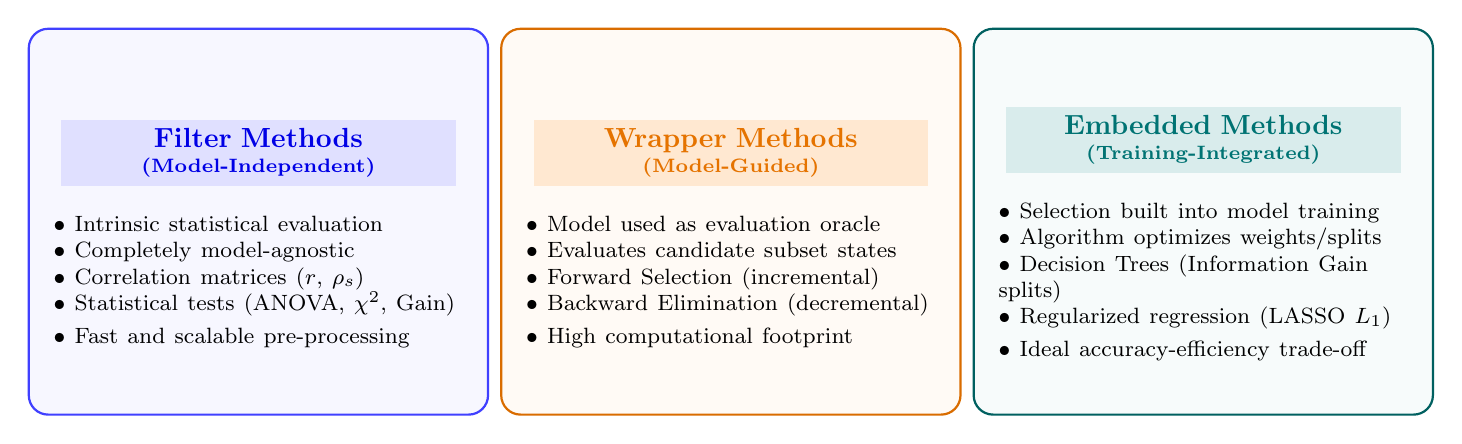
\begin{tikzpicture}[
    card/.style={
        rectangle, rounded corners=7pt, thick,
        inner sep=9pt, text width=5.2cm, minimum height=4.9cm,
        align=left
    },
    filterCard/.style={card, draw=blue!75, fill=blue!3},
    wrapperCard/.style={card, draw=orange!85!black, fill=orange!4},
    embedCard/.style={card, draw=teal!75!black, fill=teal!3}
]
    % --- 1. Filter Methods ---
    \node[filterCard] (filter) at (0, 0) {
        \begin{center}
        \colorbox{blue!12}{\parbox{4.8cm}{\centering\bfseries\color{blue!90!black} Filter Methods\\[1pt]\scriptsize (Model-Independent)}}
        \end{center}
        \vspace{2pt}
        \raggedright\footnotesize
        $\bullet$~Intrinsic statistical evaluation\\
        $\bullet$~Completely model-agnostic\\
        $\bullet$~Correlation matrices ($r$, $\rho_s$)\\
        $\bullet$~Statistical tests (ANOVA, $\chi^2$, Gain)\\
        $\bullet$~Fast and scalable pre-processing
    };

    % --- 2. Wrapper Methods ---
    \node[wrapperCard] (wrapper) at (6.0, 0) {
        \begin{center}
        \colorbox{orange!18}{\parbox{4.8cm}{\centering\bfseries\color{orange!90!black} Wrapper Methods\\[1pt]\scriptsize (Model-Guided)}}
        \end{center}
        \vspace{2pt}
        \raggedright\footnotesize
        $\bullet$~Model used as evaluation oracle\\
        $\bullet$~Evaluates candidate subset states\\
        $\bullet$~Forward Selection (incremental)\\
        $\bullet$~Backward Elimination (decremental)\\
        $\bullet$~High computational footprint
    };

    % --- 3. Embedded Methods ---
    \node[embedCard] (embed) at (12.0, 0) {
        \begin{center}
        \colorbox{teal!15}{\parbox{4.8cm}{\centering\bfseries\color{teal!90!black} Embedded Methods\\[1pt]\scriptsize (Training-Integrated)}}
        \end{center}
        \vspace{2pt}
        \raggedright\footnotesize
        $\bullet$~Selection built into model training\\
        $\bullet$~Algorithm optimizes weights/splits\\
        $\bullet$~Decision Trees (Information Gain splits)\\
        $\bullet$~Regularized regression (LASSO $L_1$)\\
        $\bullet$~Ideal accuracy-efficiency trade-off
    };
\end{tikzpicture}%
}
\caption{Schematic comparison between Filter, Wrapper, and Embedded feature selection paradigms.}
\label{fig:feature-selection-methods}
\end{figure}

\subsection{Wrapper Strategies}
Since an exhaustive search across all subsets of $p$ attributes entails evaluating $2^p$ combinations (for $p=20$, exceeding 1 million subsets), wrappers use greedy search heuristics:
\begin{itemize}
    \item \textbf{Forward Selection:} Starts from an empty set $\emptyset$. In each iteration, candidates are evaluated individually and the feature granting the largest performance gain is added. The search terminates when improvement falls below a pre-set threshold.
    \item \textbf{Backward Elimination:} Starts with all $p$ attributes. In each step, the attribute causing the least performance loss (or greatest gain) is pruned.
\end{itemize}

---

\section{Feature Creation}

\textbf{Feature creation} defines new synthetic attributes capturing latent dynamics more effectively than raw variables:

\begin{itemize}
    \item \textbf{Domain-Driven Feature Construction:} Algebraic combinations reflecting domain knowledge.
    \begin{example}[Employee Efficiency Metric]
    In workplace productivity analysis, an employee is characterized by: tasks completed per month, hours worked per month, and standard expected time per task. Instead of using raw variables in isolation, define:
    \begin{equation}
    \text{Efficiency} = \frac{\text{Hours actually spent finishing tasks}}{\text{Hours normally required to finish tasks}}
    \end{equation}
    \end{example}
    \item \textbf{Unstructured Data (Computer Vision):} Raw pixel intensities are poorly suited for linear models. High-level features (edge descriptors, color histograms, facial landmark heatmaps) are extracted instead.
    \item \textbf{Feature Projection / Extraction:} Mathematical mappings from $\mathbb{R}^p$ to $\mathbb{R}^k$ ($k < p$). Linear approaches include \textbf{Principal Component Analysis (PCA)} and \textbf{Singular Value Decomposition (SVD)}; non-linear methods include \textit{Linear Discriminant Analysis} (LDA), \textit{Non-Negative Matrix Factorization} (NMF), and neural \textit{Autoencoders}.
\end{itemize}

---

\section{Principal Component Analysis (PCA)}

\textbf{Principal Component Analysis} (PCA) is the foundational unsupervised method for linear dimensionality reduction.

\subsection{Geometric Intuition and Objectives}
Real-world attributes are often linearly dependent:
\begin{itemize}
    \item Rent expense, monthly salary, and groceries budget.
    \item Bank deposits, salary, and employment tenure.
\end{itemize}
PCA derives a new orthogonal coordinate system rotated relative to the original space:
\begin{enumerate}
    \item The \textbf{first principal component (PC1)} points along the direction of maximum projected data variance.
    \item The \textbf{second principal component (PC2)} is constrained to be strictly \textbf{orthogonal} to PC1 while capturing the maximum remaining variance.
    \item Each successive component $\text{PC}_i$ is mutually orthogonal to all preceding axes and maximizes residual dispersion.
\end{enumerate}

\subsection{Formal 5-Step Algorithmic Procedure}
Given a data matrix $\mathbf{D} \in \mathbb{R}^{m \times n}$ with $m$ observations and $n$ continuous variables:

\begin{algorithm}[H]
\caption{Principal Component Analysis (PCA)}
\KwInput{Raw data matrix $\mathbf{D} \in \mathbb{R}^{m \times n}$, target dimension $k \le n$.}
\KwOutput{Reduced matrix $\mathbf{Z} \in \mathbb{R}^{m \times k}$.}
\BlankLine
\tcp{Step 1: Centering and Standardization}
Compute column-wise sample means $\bar{x}_j = \frac{1}{m}\sum_{i=1}^m x_{ij}$\;
Subtract means to produce centered matrix $\mathbf{C} \in \mathbb{R}^{m \times n}$: $c_{ij} = x_{ij} - \bar{x}_j$\;
(Optional/Recommended): Divide by standard deviation $s_j$ when feature units differ\;
\BlankLine
\tcp{Step 2: Covariance Matrix Computation}
Compute the sample covariance matrix $\mathbf{V} \in \mathbb{R}^{n \times n}$:
\begin{equation}
\mathbf{V} = \frac{1}{m-1}\mathbf{C}^T\mathbf{C}
\end{equation}
$\mathbf{V}$ is square, symmetric ($v_{ij} = v_{ji}$), and positive semi-definite, with diagonal elements equal to feature variances\;
\BlankLine
\tcp{Step 3: Eigenvalue and Eigenvector Decomposition}
Compute orthonormal eigenvectors $\mathbf{e}_j$ and eigenvalues $\lambda_j$ by solving:
\begin{equation}
\mathbf{V}\mathbf{e}_j = \lambda_j \mathbf{e}_j \quad \text{with } \|\mathbf{e}_j\|_2 = 1
\end{equation}
\BlankLine
\tcp{Step 4: Sorting and Selection of Top $k$ Components}
Sort eigenvalues in descending order: $\lambda_1 \ge \lambda_2 \ge \cdots \ge \lambda_n \ge 0$\;
Select the top $k$ corresponding eigenvectors $\{\mathbf{e}_1, \dots, \mathbf{e}_k\}$ to form transformation matrix $\mathbf{P} \in \mathbb{R}^{n \times k}$\;
\BlankLine
\tcp{Step 5: Projection into Reduced Subspace}
Project the centered matrix into the new space:
\begin{equation}
\mathbf{Z} = \mathbf{C}\mathbf{P} \in \mathbb{R}^{m \times k}
\end{equation}
\end{algorithm}

\subsection{Significance of Covariance and Eigenvalues}
\begin{itemize}
    \item \textbf{Covariance Sign:} The sign of $\text{Cov}(x, y)$ dictates the co-variation direction:
    \begin{itemize}
        \item $\text{Cov}(x, y) > 0$: $x$ and $y$ increase or decrease together.
        \item $\text{Cov}(x, y) < 0$: as $x$ increases, $y$ tends to decrease.
        \item $\text{Cov}(x, y) \approx 0$: no linear association.
    \end{itemize}
    \item \textbf{Eigenvectors \& Eigenvalues:} Eigenvectors define the \textbf{principal axes of maximum variance}. Each eigenvalue $\lambda_j$ quantifies the variance carried by component $\text{PC}_j$.
    \item \textbf{Explained Variance Ratio:}
    \begin{equation}
    \text{Explained Variance Ratio}_j = \frac{\lambda_j}{\sum_{i=1}^n \lambda_i}
    \end{equation}
\end{itemize}

\begin{figure}[H]
\centering

\includegraphics[width=0.78\textwidth]{pca_scree_plot.pdf}
\caption{Scree plot computed on the 4 numerical attributes of the Iris dataset. The first principal component (PC1) accounts for 73.0\% of total variance, while PC1 and PC2 together cover 95.8\%, confirming the adequacy of a 2D projection.}
\label{fig:pca-scree-plot}
\end{figure}

\begin{figure}[H]
\centering

\includegraphics[width=0.82\textwidth]{pca_2d_projection.pdf}
\caption{2D PCA projection of the Iris dataset along PC1 and PC2. Unsupervised projection preserves linear separability for Setosa and clear morphological separation between Versicolor and Virginica without needing ground-truth labels.}
\label{fig:pca-2d-projection}
\end{figure}

\subsection{Python Lab: PCA and Scree Plot}
\label{subsec:lab-python-pca-en}
\begin{noteblock}{Run this section in the Interactive Notebook}
\textbf{Notebook:} \href{http://localhost:8888/lab/tree/notebooks/2_feature_engineering_and_data_representation.ipynb}{\texttt{2\_feature\_engineering\_\dots.ipynb}} \hfill \href{http://localhost:8888/lab/tree/notebooks/2_feature_engineering_and_data_representation.ipynb}{\textbf{[Open in Jupyter Lab]}} \\
\textit{Local server:} \url{http://localhost:8888} \quad (launch command: \texttt{docker compose up jupyter})
\end{noteblock}
In the companion notebook \texttt{2\_feature\_engineering\_\dots.ipynb}, unsupervised dimensionality reduction via PCA, eigenvalue variance decomposition, and the Scree Plot are implemented using Scikit-learn as shown in Listing~\ref{lst:python-pca-en}:

\begin{lstlisting}[language=Python, style=code, caption={PCA execution, eigenvalue variance decomposition, and Scree Plot with Scikit-learn.}, label={lst:python-pca-en}]
import pandas as pd
import numpy as np
import matplotlib.pyplot as plt
from sklearn.decomposition import PCA

df = pd.read_csv('./data_notebook/data/correct_tips.csv', index_col=0)
numeric_cols = ['total_bill', 'tip', 'size', 'age']
X = df[numeric_cols]

# 1. Instantiate and fit full PCA model
pca = PCA()
X_pca = pca.fit_transform(X)

# 2. Extract eigenvalues (explained variance) and variance ratios
eigenvalues = pca.explained_variance_
var_ratio = pca.explained_variance_ratio_
cum_var = np.cumsum(var_ratio)

for i, (eig, ratio, c) in enumerate(zip(eigenvalues, var_ratio, cum_var), 1):
    print(f"PC{i}: Eigenvalue={eig:.3f} | Variance={ratio*100:.1f}% | Cumulative={c*100:.1f}%")

# 3. Scree Plot of principal component eigenvalues
plt.figure(figsize=(7, 4))
plt.plot(range(1, len(eigenvalues) + 1), eigenvalues, marker='o', linestyle='--', color='b')
plt.title("Scree Plot: Principal Component Eigenvalues")
plt.xlabel("Principal Component")
plt.ylabel("Eigenvalue (Explained Variance)")
plt.grid(True)
plt.show()
\end{lstlisting}

\section{Missing Value and Anomaly Cleaning}

\subsection{Types and Origins of Data Anomalies}
Raw datasets frequently suffer from collection imperfections caused by hardware sensor faults, survey non-responses, data transcription errors, or evolving logging formats:
\begin{itemize}
    \item \textbf{Missing Values:} Explicit unrecorded fields represented as \texttt{NULL} or \texttt{NaN}.
    \item \textbf{Unknown Values:} Populated records lacking verifiable real-world semantic meaning.
    \item \textbf{Invalid Values:} Entries violating domain integrity constraints (e.g., negative ages, impossible exam grades, or corrupted identifier strings).
\end{itemize}

\subsection{Methodological Strategies for Missing Data Handling}
In practical data mining workflows, missing data remediation falls into three complementary approaches:

\begin{enumerate}
    \item \textbf{Elimination (\textit{Data / Attribute Removal}):}
    \begin{itemize}
        \item \textit{Listwise / Case Deletion:} Removing entire records containing one or more null attributes. This is only admissible when missing rates are negligible ($< 3\div 5\%$) and data is Missing Completely at Random (MCAR). Otherwise, discarding records introduces severe selection bias.
        \item \textit{Feature Deletion:} Dropping entire columns. Recommended when an attribute has excessive missingness (exceeding $50\div 60\%$) and possesses low predictive or explanatory relevance.
        \item \textit{Pairwise Deletion:} Used during bivariate statistical computations (such as covariance or correlation matrices) by omitting only instances lacking both attributes, thereby preserving available sample size.
    \end{itemize}

    \item \textbf{Value Imputation (\textit{Value Estimation}):}
    \begin{itemize}
        \item \textbf{Global Estimators (Mean, Median, Mode):}
        The arithmetic mean is used for symmetric continuous attributes; the median is standard for skewed distributions with heavy tails and outliers; the mode is applied to categorical features. \textit{Drawback:} artifically dampens attribute variance and attenuates cross-feature covariances.
        \item \textbf{Empirical Probability Distribution Sampling:}
        Replacement values are drawn randomly according to the observed empirical frequency distribution of valid observations. \textit{Benefit:} preserves original empirical dispersion, variance, and distributional shape.
        \item \textbf{Stratified Imputation across Segments or Clusters:}
        Data is grouped by target class, demographic segment, or unsupervised clusters (e.g., k-means); missing entries are replaced by the mean or median computed strictly within that subgroup (e.g., imputing missing salary using the median salary of the subject's exact job title).
        \item \textbf{Supervised Predictive Modeling:}
        The incomplete feature is framed as target variable $Y$. A predictive model (decision tree, linear regression, or $k$-NN) is trained on complete features to infer missing entries with maximal contextual accuracy.
    \end{itemize}

    \item \textbf{Direct Algorithmic Tolerance (\textit{Ignore Missing Values}):}
    Several data mining algorithms naturally accommodate missing entries during training without preprocessing:
    \begin{itemize}
        \item \textit{Decision Trees (e.g., C4.5):} During node splitting, instances with missing values are partitioned proportionally across child branches according to observed frequencies, or directed to a dedicated missing branch.
        \item \textit{Association Rules:} In binary transaction matrices, an absent value intrinsically represents item non-purchase ($0$), seamlessly aligning with the algorithm's operational semantics.
    \end{itemize}
\end{enumerate}

\begin{figure}[H]
\centering
\resizebox{0.98\linewidth}{!}{%
\begin{tikzpicture}[
    header/.style={rectangle, draw=blue!60, fill=blue!12, minimum width=0.95cm, minimum height=0.50cm, font=\scriptsize\bfseries, text=blue!90!black, align=center},
    cell/.style={rectangle, draw=gray!40, fill=white, minimum width=0.95cm, minimum height=0.46cm, font=\scriptsize, align=center},
    nanCell/.style={rectangle, draw=red!70, fill=red!18, minimum width=0.95cm, minimum height=0.46cm, font=\scriptsize\bfseries, text=red!80!black, align=center},
    impCell/.style={rectangle, draw=teal!70, fill=teal!18, minimum width=0.95cm, minimum height=0.46cm, font=\scriptsize\bfseries, text=teal!90!black, align=center},
    boxTitle/.style={font=\small\bfseries, text=gray!90!black, align=center},
    arrowLbl/.style={font=\scriptsize\bfseries, fill=white, inner sep=2.5pt, rounded corners=3pt}
]
    % --- Matrice Originale ---
    \node[boxTitle] (t0) at (0, 2.2) {Dataset with Missing Entries};
    \node[header] (h1) at (-0.95, 1.5) {$A_1$};
    \node[header] (h2) at (0, 1.5) {$A_2$};
    \node[header] (h3) at (0.95, 1.5) {$A_3$};

    \node[cell] at (-0.95, 0.95) {24}; \node[cell] at (0, 0.95) {1.8}; \node[cell] at (0.95, 0.95) {50};
    \node[cell] at (-0.95, 0.45) {31}; \node[nanCell] at (0, 0.45) {NaN}; \node[cell] at (0.95, 0.45) {65};
    \node[cell] at (-0.95, -0.05) {45}; \node[cell] at (0, -0.05) {2.3}; \node[cell] at (0.95, -0.05) {80};
    \node[cell] at (-0.95, -0.55) {19}; \node[nanCell] at (0, -0.55) {NaN}; \node[nanCell] at (0.95, -0.55) {NaN};
    \node[cell] at (-0.95, -1.05) {29}; \node[cell] at (0, -1.05) {1.5}; \node[cell] at (0.95, -1.05) {55};

    \draw[rounded corners=6pt, draw=blue!40, thick, fill=blue!1, fill opacity=0.3] (-1.65, -1.40) rectangle (1.65, 1.85);

    % --- Frecce alle 3 Strategie ---
    \draw[-Stealth, line width=1.3pt, color=orange!85!black] (1.75, 0.95) -- (4.4, 2.85) 
        node[midway, above=2pt, sloped, arrowLbl, draw=orange!40, text=orange!90!black] {Listwise Deletion};
        
    \draw[-Stealth, line width=1.3pt, color=red!80!black] (1.75, 0.0) -- (4.4, 0.0) 
        node[midway, above=2pt, arrowLbl, draw=red!40, text=red!85!black] {Feature Deletion};
        
    \draw[-Stealth, line width=1.3pt, color=teal!85!black] (1.75, -0.95) -- (4.4, -2.85) 
        node[midway, below=2pt, sloped, arrowLbl, draw=teal!40, text=teal!90!black] {Value Imputation};

    % --- Strategia 1: Listwise Deletion ---
    \begin{scope}[shift={(6.7, 2.95)}]
        \draw[rounded corners=7pt, draw=orange!55, fill=orange!3, thick] (-2.1, -1.35) rectangle (10.6, 1.35);
        \node[font=\footnotesize\bfseries, text=orange!95!black, anchor=west] at (-1.9, 0.98) {1. Record Elimination (\textit{Listwise Deletion})};
        
        \node[header] at (-1.1, 0.30) {$A_1$}; \node[header] at (-0.15, 0.30) {$A_2$}; \node[header] at (0.8, 0.30) {$A_3$};
        \node[cell] at (-1.1, -0.20) {24}; \node[cell] at (-0.15, -0.20) {1.8}; \node[cell] at (0.8, -0.20) {50};
        \node[cell] at (-1.1, -0.70) {45}; \node[cell] at (-0.15, -0.70) {2.3}; \node[cell] at (0.8, -0.70) {80};
        
        \draw[gray!30, line width=0.7pt] (1.45, -1.05) -- (1.45, 0.75);

        \node[font=\scriptsize, text=gray!85!black, anchor=west, align=left, text width=8.6cm] at (1.65, -0.20) {
            $\bullet$ Discards any row containing at least one missing entry (NaN)\\[5pt]
            $\bullet$ Admissible only if missing entries are rare ($< 3\div 5\%$)\\[5pt]
            $\bullet$ Severe risk of systematic \textbf{selection bias} if not MCAR
        };
    \end{scope}

    % --- Strategia 2: Feature Deletion ---
    \begin{scope}[shift={(6.7, 0.0)}]
        \draw[rounded corners=7pt, draw=red!55, fill=red!3, thick] (-2.1, -1.35) rectangle (10.6, 1.35);
        \node[font=\footnotesize\bfseries, text=red!90!black, anchor=west] at (-1.9, 0.98) {2. Attribute Elimination (\textit{Feature Deletion})};
        
        \node[header] at (-0.65, 0.30) {$A_1$}; \node[header] at (0.35, 0.30) {$A_3$};
        \node[cell] at (-0.65, -0.20) {24}; \node[cell] at (0.35, -0.20) {50};
        \node[cell] at (-0.65, -0.70) {31}; \node[cell] at (0.35, -0.70) {65};
        
        \draw[gray!30, line width=0.7pt] (1.45, -1.05) -- (1.45, 0.75);

        \node[font=\scriptsize, text=gray!85!black, anchor=west, align=left, text width=8.6cm] at (1.65, -0.20) {
            $\bullet$ Drops incomplete feature ($A_2$) entirely from predictor set\\[5pt]
            $\bullet$ Recommended if missing proportion is critical ($> 50\div 60\%$)\\[5pt]
            $\bullet$ Preserves all remaining observations in the dataset
        };
    \end{scope}

    % --- Strategia 3: Value Imputation ---
    \begin{scope}[shift={(6.7, -2.95)}]
        \draw[rounded corners=7pt, draw=teal!55, fill=teal!3, thick] (-2.1, -1.35) rectangle (10.6, 1.35);
        \node[font=\footnotesize\bfseries, text=teal!90!black, anchor=west] at (-1.9, 0.98) {3. Value Imputation (\textit{Value Estimation})};
        
        \node[header] at (-1.1, 0.30) {$A_1$}; \node[header] at (-0.15, 0.30) {$A_2$}; \node[header] at (0.8, 0.30) {$A_3$};
        \node[cell] at (-1.1, -0.20) {31}; \node[impCell] at (-0.15, -0.20) {1.9}; \node[cell] at (0.8, -0.20) {65};
        \node[cell] at (-1.1, -0.70) {19}; \node[impCell] at (-0.15, -0.70) {1.9}; \node[impCell] at (0.8, -0.70) {58};
        
        \draw[gray!30, line width=0.7pt] (1.45, -1.05) -- (1.45, 0.75);

        \node[font=\scriptsize, text=gray!85!black, anchor=west, align=left, text width=8.6cm] at (1.65, -0.20) {
            $\bullet$ Replacement by mean, median or regression/$k$-NN model\\[5pt]
            $\bullet$ \textbf{Empirical sampling}: preserves original variance\\[5pt]
            $\bullet$ \textbf{Stratified imputation}: preserves cross-cluster nuances
        };
    \end{scope}
\end{tikzpicture}%
}
\caption{Schematic overview of missing value management strategies: record or attribute elimination versus value imputation.}
\label{fig:missing-values-strategies}
\end{figure}

\subsection{Univariate Outlier Detection and Treatment}
In preprocessing workflows, analysts deploy two formal criteria (Figure~\ref{fig:outlier-detection-methods}):
\begin{enumerate}
    \item \textbf{Tukey Interquartile Range (IQR) Fences:}
    \begin{equation}
    \text{IQR} = Q_3 - Q_1, \quad L = Q_1 - 1.5 \times \text{IQR}, \quad U = Q_3 + 1.5 \times \text{IQR}
    \end{equation}
    An observation $x$ is an outlier if $x < L$ or $x > U$.
    \begin{itemize}
        \item \textit{Winsorization:} Capping values at $L$ or $U$.
        \item \textit{Median Replacement:} Overwriting outliers with $Q_2$.
    \end{itemize}
    \item \textbf{Parametric Z-Score Approach:}
    For normally distributed data:
    \begin{itemize}
        \item 95\% of observations fall within $[ -1.96, +1.96 ]$.
        \item 99\% fall within $[ -2.58, +2.58 ]$.
        \item Standard extreme outlier threshold: $|z| > 3.29$ (probability $< 0.1\%$).
        \item \textit{Outlier treatment:} Truncating to $z = \pm 3.0$ or replacing with the mean ($z = 0$).
    \end{itemize}
\end{enumerate}

\begin{figure}[H]
\centering
\resizebox{0.96\linewidth}{!}{%
\begin{tikzpicture}[
    outlierPt/.style={circle, draw=red!80!black, fill=red!45, inner sep=2.2pt, thick},
    whisker/.style={line width=1.1pt, draw=blue!85!black},
    boxStyle/.style={rectangle, draw=blue!85!black, line width=1.2pt, fill=blue!10}
]
    % --- SEZIONE A: BOXPLOT TUKEY ---
    \node[anchor=west, font=\small\bfseries, text=blue!90!black] at (-6.8, 4.4) {A) Non-Parametric Interquartile Range Rule (Tukey IQR Fences)};

    % Asse orizzontale
    \draw[-Stealth, line width=0.8pt, color=gray!70] (-6.8, 1.8) -- (6.8, 1.8) node[right, font=\scriptsize] {$x$};
    \foreach \x in {-5.5, -3.5, -1.0, 0.5, 2.0, 4.5, 5.5} {
        \draw[gray!60] (\x, 1.7) -- (\x, 1.9);
    }
    
    % Etichette sotto l'asse alternate per leggibilità
    \node[below=3pt, font=\scriptsize\bfseries, text=red!80!black] at (-3.5, 1.7) {$L = Q_1 - 1.5\,\text{IQR}$};
    \node[below=3pt, font=\scriptsize\bfseries, text=red!80!black] at (4.5, 1.7) {$U = Q_3 + 1.5\,\text{IQR}$};
    \node[below=3pt, font=\scriptsize] at (-1.0, 1.7) {$Q_1$};
    \node[below=3pt, font=\scriptsize\bfseries, text=blue!90!black] at (0.5, 1.7) {Median ($Q_2$)};
    \node[below=3pt, font=\scriptsize] at (2.0, 1.7) {$Q_3$};

    % Box
    \draw[boxStyle] (-1.0, 2.3) rectangle (2.0, 3.3);
    \draw[line width=1.6pt, draw=blue!95!black] (0.5, 2.3) -- (0.5, 3.3);

    % Staffa IQR SOPRA il box
    \draw[decorate, decoration={brace, amplitude=4pt}, line width=0.8pt, draw=blue!80!black] (-1.0, 3.4) -- (2.0, 3.4) 
        node[midway, above=4pt, font=\scriptsize\bfseries, text=blue!85!black] {$\text{IQR} = Q_3 - Q_1$};

    % Baffi (Whiskers)
    \draw[whisker] (-1.0, 2.8) -- (-3.5, 2.8);
    \draw[whisker] (-3.5, 2.5) -- (-3.5, 3.1);
    \draw[whisker] (2.0, 2.8) -- (4.5, 2.8);
    \draw[whisker] (4.5, 2.5) -- (4.5, 3.1);

    % Punti Outlier
    \node[outlierPt] at (-4.8, 2.8) {};
    \node[outlierPt] at (-5.6, 2.8) {};
    \node[outlierPt] at (5.2, 2.8) {};
    \node[outlierPt] at (6.0, 2.8) {};

    \node[font=\scriptsize\bfseries, text=red!80!black] at (-5.2, 3.5) {Outlier ($x < L$)};
    \node[font=\scriptsize\bfseries, text=red!80!black] at (5.6, 3.5) {Outlier ($x > U$)};

    % Frecce Winsorizing
    \draw[-Stealth, line width=1pt, draw=teal!80!black, dashed] (-5.2, 2.4) to[bend left=18] 
        node[midway, below=1pt, font=\tiny\bfseries, text=teal!90!black] {Winsorizing $\to L$} (-3.55, 2.4);
    \draw[-Stealth, line width=1pt, draw=teal!80!black, dashed] (5.6, 2.4) to[bend right=18] 
        node[midway, below=1pt, font=\tiny\bfseries, text=teal!90!black] {Winsorizing $\to U$} (4.55, 2.4);

    % --- SEPARATORE ---
    \draw[dashed, color=gray!30] (-6.8, 0.8) -- (6.8, 0.8);

    % --- SEZIONE B: CURVA NORMALE Z-SCORE ---
    \node[anchor=west, font=\small\bfseries, text=purple!85!black] at (-6.8, 0.4) {B) Parametric Z-Score Rule (Gaussian Distribution $\mathcal{N}(\mu, \sigma^2)$)};

    % Asse orizzontale z-score (a y = -3.0)
    \draw[-Stealth, line width=0.8pt, color=gray!70] (-6.8, -3.0) -- (6.8, -3.0) node[right, font=\scriptsize] {$z$};

    % Area 95% (da -1.96 a +1.96)
    \fill[teal!15] (-2.0, -3.0) .. controls (-1.0, -2.9) and (-0.8, -1.0) .. (0, -0.6)
                                .. controls (0.8, -1.0) and (1.0, -2.9) .. (2.0, -3.0) -- cycle;

    % Area Outlier Sinistra (z < -3.29)
    \fill[red!30] (-6.2, -3.0) -- (-3.3, -3.0) .. controls (-3.8, -2.94) and (-4.8, -2.98) .. (-6.2, -3.0) -- cycle;
    % Area Outlier Destra (z > 3.29)
    \fill[red!30] (3.3, -3.0) .. controls (4.8, -2.98) and (3.8, -2.94) .. (6.2, -3.0) -- (3.3, -3.0) -- cycle;

    % Curva Gaussiana completa disegnata con Bézier smooth
    \draw[line width=1.4pt, color=purple!85!black] 
        (-6.2, -3.0) .. controls (-4.5, -2.98) and (-3.0, -2.8) .. (-2.0, -2.2)
                     .. controls (-1.2, -1.6) and (-0.6, -0.7) .. (0, -0.6)
                     .. controls (0.6, -0.7) and (1.2, -1.6) .. (2.0, -2.2)
                     .. controls (3.0, -2.8) and (4.5, -2.98) .. (6.2, -3.0);

    % Linee verticali
    \draw[line width=0.9pt, color=purple!80!black, dashed] (0, -3.0) -- (0, -0.6) 
        node[above=2pt, font=\scriptsize\bfseries] {$\mu$ ($z=0$)};
    \draw[line width=0.8pt, color=teal!70!black, dotted] (-2.0, -3.0) -- (-2.0, -2.2);
    \draw[line width=0.8pt, color=teal!70!black, dotted] (2.0, -3.0) -- (2.0, -2.2);
    \draw[line width=1pt, color=red!70!black, dashed] (-3.3, -3.0) -- (-3.3, -2.85);
    \draw[line width=1pt, color=red!70!black, dashed] (3.3, -3.0) -- (3.3, -2.85);

    % Etichette
    \node[font=\scriptsize\bfseries, text=teal!90!black] at (0, -1.6) {95\% of the population};
    \node[font=\tiny, text=gray!80!black] at (0, -2.0) {($-1.96 \le z \le +1.96$)};

    \node[below=2pt, font=\scriptsize\bfseries, text=red!80!black] at (-3.3, -3.0) {$-3.29$};
    \node[below=2pt, font=\scriptsize\bfseries, text=red!80!black] at (3.3, -3.0) {$+3.29$};
    \node[below=2pt, font=\scriptsize, text=teal!80!black] at (-2.0, -3.0) {$-1.96$};
    \node[below=2pt, font=\scriptsize, text=teal!80!black] at (2.0, -3.0) {$+1.96$};
    \node[below=2pt, font=\scriptsize\bfseries] at (0, -3.0) {$0$};

    \node[font=\scriptsize\bfseries, text=red!85!black, align=center] at (-4.7, -1.8) {Extreme Outliers\\$|z| > 3.29$\\($p < 0.1\%$)};
    \node[font=\scriptsize\bfseries, text=red!85!black, align=center] at (4.7, -1.8) {Extreme Outliers\\$|z| > 3.29$\\($p < 0.1\%$)};
\end{tikzpicture}%
}
\caption{Comparison of univariate outlier detection methods: non-parametric Tukey IQR fences versus parametric Gaussian Z-Score rule.}
\label{fig:outlier-detection-methods}
\end{figure}

\FloatBarrier

\section{Discretization and Binarization}

\subsection{Definition and Benefits of Discretization}
\textbf{Discretization} converts a continuous attribute into an ordinal discrete attribute by binning infinite real values into $k$ categorical intervals.

\begin{itemize}
    \item \textbf{Interpretability:} Produces concise categories (such as Young, Adult, Senior).
    \item \textbf{Robustness:} Attenuates measurement noise and isolated outliers.
    \item \textbf{Algorithm Compatibility:} Required by associative rule algorithms and specific naive Bayes models.
\end{itemize}

\subsection{Unsupervised Discretization (Binning)}
\begin{enumerate}
    \item \textbf{Equal-Width (Natural) Binning:}
    Partitions data range into $k$ equal-width intervals $\delta$:
    \begin{equation}
    \delta = \frac{x_{\max} - x_{\min}}{k}
    \end{equation}
    Value $x_j$ belongs to interval $i \in \{0, \dots, k-1\}$ if:
    \begin{equation}
    x_j \in [x_{\min} + i\delta, \; x_{\min} + (i+1)\delta)
    \end{equation}
    \textit{Drawback:} Heavily skewed data clusters into a few bins, leaving others nearly empty.

    \item \textbf{Equal-Frequency (Quantile) Binning:}
    Partitions sorted data into $k$ bins containing roughly equal counts $f = \frac{N}{k}$:
    Sorted element $x_i$ ($i \in \{0, \dots, N-1\}$) falls into bin $j$ if:
    \begin{equation}
    j \times f \le i < (j+1) \times f
    \end{equation}
    \textit{Advantage:} Maximizes bin entropy and avoids empty partitions.
\end{enumerate}

\subsection{Criteria for Choosing Number of Bins}
\begin{itemize}
    \item \textbf{Sturges' Rule (1929):} Recommended for symmetric unimodal distributions:
    \begin{equation}
    k = 1 + \frac{10}{3} \log_{10}(N) \approx 1 + 3.322 \log_{10}(N) = 1 + \log_2(N)
    \end{equation}
    \item \textbf{Scott's Rule (1979):} Directly calculates optimal bin width $h$ based on sample standard deviation $s$:
    \begin{equation}
    h = \frac{3.5 \times s}{\sqrt[3]{N}}
    \end{equation}
\end{itemize}

\subsection{Supervised Discretization: Entropy-Based Splitting}
In supervised classification, discretization maximizes \textbf{class purity} within intervals by minimizing conditional class entropy.
\begin{enumerate}
    \item Evaluates candidate split thresholds $T$ along the sorted range of feature $X$.
    \item For partitions $S_1 = \{x \le T\}$ and $S_2 = \{x > T\}$, computes weighted entropy:
    \begin{equation}
    E(X, T) = \frac{|S_1|}{|S|} \text{Entropy}(S_1) + \frac{|S_2|}{|S|} \text{Entropy}(S_2)
    \end{equation}
    where $\text{Entropy}(S) = -\sum_{c=1}^C p_c \log_2(p_c)$.
    \item Selects threshold $T^*$ that maximizes Information Gain ($E(X) - E(X, T)$).
    \item Recursively splits the interval with highest entropy until reaching a target bin count or stopping criterion.
\end{enumerate}

\subsection{Binarization}
\textbf{Binarization} maps continuous attributes (following discretization) or categorical attributes into one or more binary variables ($0$ or $1$). Data mining literature contrasts two primary paradigms:

\begin{enumerate}
    \item \textbf{Compact Positional Binary Encoding (\textit{Integer-to-Binary}):}
    A categorical attribute with $m$ distinct categories is mapped to integers $\{0, 1, \dots, m-1\}$ and expressed in base-$2$ positional format using $k = \lceil \log_2(m) \rceil$ bits.
    \begin{itemize}
        \item \textit{Example:} For a feature with $m=4$ states (e.g.~Red, Blue, Green, Yellow), $\lceil \log_2(4) \rceil = 2$ bits are needed:
        \begin{equation}
        \text{Red} \to 00_2, \quad \text{Blue} \to 01_2, \quad \text{Green} \to 10_2, \quad \text{Yellow} \to 11_2
        \end{equation}
        \item \textit{Critical Deficiencies and Side Effects:} While space-efficient, positional encoding introduces \textbf{entirely artificial metric distances and spurious correlations}:
        \begin{itemize}
            \item \textit{Distorted Distance:} The Hamming distance between Red ($00$) and Blue ($01$) is $1$, whereas between Red ($00$) and Yellow ($11$) it is $2$. Machine learning models erroneously perceive Yellow as ``twice as far'' from Red as Blue, violating nominal symmetry.
            \item \textit{Spurious Correlations:} Accidental bit sharing (e.g., the leading bit $1$ shared by Green and Yellow) creates artificial linear relationships between synthetic coordinates.
        \end{itemize}
    \end{itemize}

    \item \textbf{Asymmetric Binarization / One-Hot Encoding:}
    For a feature with $m$ categories, $m$ distinct binary indicators $x_1, \dots, x_m$ are introduced, where $x_j = 1$ if the instance assumes modality $j$, and $x_j = 0$ otherwise (Table~\ref{tab:binarization-example}).
    \begin{itemize}
        \item \textit{Geometric Invariance:} All categories are mutually orthogonal in $\mathbb{R}^m$ and equidistant ($\|\mathbf{x}_i - \mathbf{x}_j\|_2 = \sqrt{2}$ for $i \ne j$), preserving the unranked nature of nominal variables.
        \item \textit{Core Requirement for Association Analysis (Association Rules):}
        Frequent pattern mining algorithms (such as Apriori or FP-Growth) model transactions as sets of asymmetric binary items:
        \begin{itemize}
            \item Item presence ($1$, e.g., ``the customer bought \texttt{Bread}'') conveys active discriminative information and contributes to support and confidence.
            \item Item absence ($0$) constitutes the passive, non-informative background state (in a supermarket catalog of $50\,000$ products, each basket contains very few items).
            \item With symmetric binary encoding or compact positional bits, algorithms would extract billions of uninformative or misleading associations based on joint non-presence (e.g., ``customers who do not buy caviar do not buy helicopters''). One-Hot encoding isolates each feature level as an independent asymmetric item.
        \end{itemize}
    \end{itemize}
\end{enumerate}

\begin{table}[H]
\centering
\small
\begin{tabular}{lcccccc}
\toprule
\textbf{Categorical Value} & \textbf{Index} & $x_1$ & $x_2$ & $x_3$ & $x_4$ & $x_5$ \\
\midrule
awful  & 0 & 1 & 0 & 0 & 0 & 0 \\
poor   & 1 & 0 & 1 & 0 & 0 & 0 \\
OK     & 2 & 0 & 0 & 1 & 0 & 0 \\
good   & 3 & 0 & 0 & 0 & 1 & 0 \\
great  & 4 & 0 & 0 & 0 & 0 & 1 \\
\bottomrule
\end{tabular}
\caption{One-Hot Encoding of a categorical attribute with $m=5$ states into $5$ asymmetric binary indicator attributes.}
\label{tab:binarization-example}
\end{table}

\subsection{Python Lab: Discretization and Categorical Encoding}
\label{subsec:lab-python-encoding-en}
\begin{noteblock}{Run this section in the Interactive Notebook}
\textbf{Notebook:} \href{http://localhost:8888/lab/tree/notebooks/2_feature_engineering_and_data_representation.ipynb}{\texttt{2\_feature\_engineering\_\dots.ipynb}} \hfill \href{http://localhost:8888/lab/tree/notebooks/2_feature_engineering_and_data_representation.ipynb}{\textbf{[Open in Jupyter Lab]}} \\
\textit{Local server:} \url{http://localhost:8888} \quad (launch command: \texttt{docker compose up jupyter})
\end{noteblock}
In the companion notebook \texttt{2\_feature\_engineering\_\dots.ipynb}, continuous attribute discretization and categorical encoding strategies (One-Hot Encoding and Target Encoding) are implemented using Scikit-learn as displayed in Listing~\ref{lst:python-encoding-en}:

\begin{lstlisting}[language=Python, style=code, caption={Discretization with KBinsDiscretizer and Categorical Encoding (One-Hot and Target Encoding) with Scikit-learn.}, label={lst:python-encoding-en}]
import pandas as pd
from sklearn.preprocessing import KBinsDiscretizer, OneHotEncoder, TargetEncoder

df = pd.read_csv('./data_notebook/data/correct_tips.csv', index_col=0)

# 1. Continuous to ordinal discretization (Equal-Width vs Equal-Frequency)
kbins_uniform = KBinsDiscretizer(n_bins=4, encode='ordinal', strategy='uniform')
df['bill_uniform'] = kbins_uniform.fit_transform(df[['total_bill']])

kbins_quantile = KBinsDiscretizer(n_bins=4, encode='ordinal', strategy='quantile')
df['bill_quantile'] = kbins_quantile.fit_transform(df[['total_bill']])
print("Uniform bin frequencies:\n", df['bill_uniform'].value_counts())

# 2. One-Hot Encoding for nominal categorical features
ohe = OneHotEncoder(handle_unknown='ignore', sparse_output=False)
ohe_day = ohe.fit_transform(df[['day']])
df_ohe = pd.DataFrame(ohe_day, columns=ohe.get_feature_names_out(['day']))
print("Generated One-Hot features:\n", df_ohe.head(3))

# 3. Supervised Target Encoding
target_encoder = TargetEncoder(smooth="auto")
# Estimates smoothed conditional expected target value ('tip') per category
df['day_target_encoded'] = target_encoder.fit_transform(df[['day']], df['tip'])
print(df[['day', 'day_target_encoded']].drop_duplicates())
\end{lstlisting}

\FloatBarrier

---

\section{Attribute Transformation and Variance Stabilization}

\subsection{Motivations and Formal Properties}
An attribute transformation is a mapping $T: \mathcal{X} \to \mathcal{Y}$ replacing original value $x$ with $y = T(x)$. Desirable properties include:
\begin{enumerate}
    \item \textbf{Information Preservation:} Preserves natural monotonic ordering ($x_a < x_b \implies T(x_a) < T(x_b)$).
    \item \textbf{Distribution Normalization:} Transforms skewed distributions into approximately normal, symmetric shapes.
    \item \textbf{Linearization:} Straightens nonlinear bivariate relationships.
    \item \textbf{Analytical Regularity:} Continuous, differentiable, and invertible mappings.
\end{enumerate}

\subsection{Exponential and Logarithmic Transformation Families}
The general parametric transformation for $x > 0$ is defined as:
\begin{equation}
T_p(x) = \begin{cases}
a x^p + b & \text{if } p \ne 0 \\
c \log(x) + d & \text{if } p = 0
\end{cases}
\end{equation}
Depending on parameter $p$:
\begin{itemize}
    \item \textbf{Linear Transformation ($p=1$):} Preserves skewness and correlation exactly; used for unit scaling:
    \begin{itemize}
        \item Currency conversion: $\text{Lira} = 1936.27 \times \text{Euro}$, with $p=1, a=1936.27, b=0$.
        \item Temperature conversion: $^\circ\text{C} = \frac{5}{9}(^\circ\text{F} - 32) \quad (p=1, a=5/9, b=-160/9)$.
    \end{itemize}
    \item \textbf{Logarithmic Transformation ($p=0$):} Applicable to positive values $x > 0$ under the general specification $T(x) = c \log(x) + d$. Compresses long right tails in log-normal distributions, stabilizing variance and mitigating extreme outliers.
    \begin{remark}[Logarithms and Seasonality]
    Logarithmic transformations do not eliminate seasonal cycles, but compress amplitude fluctuations that scale with the series level.
    \end{remark}

    \begin{example}[Logarithmic Transformation on Sparse Data: Bar and Beer Example]
    Consider the lecture case study (Table~\ref{tab:bar-beer-gain}), analyzing sales earnings (\textit{Gain}) across beer brands in different commercial bars.

    \begin{table}[H]
    \centering
    \small
    \begin{tabular}{llrr}
    \toprule
    \textbf{Bar} & \textbf{Beer Brand} & \textbf{Original Gain} & \textbf{Transformed Gain } $\log_{10}(\text{Gain})$ \\
    \midrule
    Bar A & Bud   & 20    & 1.3010 \\
    Bar A & Becks & 10000 & 4.0000 \\
    Bar C & Bud   & 300   & 2.4771 \\
    Bar D & Bud   & 400   & 2.6021 \\
    Bar D & Becks & 5     & 0.6990 \\
    Bar E & Becks & 120   & 2.0792 \\
    Bar E & Bud   & 120   & 2.0792 \\
    Bar F & Bud   & 11000 & 4.0414 \\
    Bar G & Bud   & 1300  & 3.1139 \\
    Bar H & Bud   & 3200  & 3.5051 \\
    Bar H & Becks & 1000  & 3.0000 \\
    Bar I & Bud   & 135   & 2.1303 \\
    \bottomrule
    \end{tabular}
    \caption{Effect of logarithmic transformation ($\log_{10}$) on beer sales across bars: compression of severe dispersion.}
    \label{tab:bar-beer-gain}
    \end{table}

    \textbf{Statistical Diagnosis and Compression of Sparse Data:}
    \begin{itemize}
        \item \textit{Raw Series:} Sample mean $\bar{x} \approx 2481.82$, Standard deviation $s \approx 4079.02$, Minimum $5$, $1^{\text{st}}$ Quartile $120$, Median $400$, $3^{\text{rd}}$ Quartile $2250$, Maximum $11000$. The standard deviation substantially exceeds the mean ($s > \bar{x}$) and the maximum spans over three orders of magnitude above the minimum ($2200 \times$). Data is heavily skewed and sparse in the upper range (\textit{``Data are sparse!''}), severely distorting distance metrics and regression loss functions.
        \item \textit{Transformed Series:} Applying $y = \log_{10}(\text{Gain})$ maps the entire dynamic range into the interval $[0.6990, 4.0414]$. Multiplicative scales (orders of magnitude) become uniform linear intervals, stabilizing variance and restoring distributional balance (Figure~\ref{fig:log-transform-compression}).
    \end{itemize}
    \end{example}

    \begin{figure}[H]
    \centering
    \resizebox{0.96\linewidth}{!}{%
    \begin{tikzpicture}[
        dotRaw/.style={circle, draw=orange!80!black, fill=orange!50, inner sep=2.3pt, thick},
        dotLog/.style={circle, draw=teal!80!black, fill=teal!50, inner sep=2.3pt, thick},
        axisLine/.style={-Stealth, line width=0.9pt, color=gray!75}
    ]
        % --- SECTION A: RAW LINEAR SCALE ---
        \node[anchor=west, font=\small\bfseries, text=orange!90!black] at (-0.5, 5.0) {A) Natural Linear Scale (Raw Sales $x \in [5, 11000]$) --- \textit{Hyper-Sparse Space}};
        
        % Diagnostic summary box
        \node[font=\scriptsize\bfseries, text=red!80!black, fill=red!6, draw=red!35, rounded corners=3pt, inner sep=3.5pt] at (6.0, 4.3) {
            Diagnosis: \textit{``Data are sparse!''} --- Variance dominated by extreme isolated spikes ($s \approx 4079 > \bar{x}$)
        };

        % x-axis from 0 to 11500 (mapped to x = 0 to 11.5)
        \draw[axisLine] (0, 2.3) -- (12.2, 2.3) node[right, font=\scriptsize] {Gain};
        \foreach \val/\x in {0/0, 2000/2.0, 4000/4.0, 6000/6.0, 8000/8.0, 10000/10.0} {
            \draw[gray!60] (\x, 2.2) -- (\x, 2.4);
            \node[below=3pt, font=\tiny, text=gray!80!black] at (\x, 2.2) {\val};
        }
        
        % Raw points
        \node[dotRaw] at (0.005, 2.3) {};
        \node[dotRaw] at (0.02, 2.3) {};
        \node[dotRaw] at (0.12, 2.3) {};
        \node[dotRaw] at (0.135, 2.3) {};
        \node[dotRaw] at (0.30, 2.3) {};
        \node[dotRaw] at (0.40, 2.3) {};
        \node[dotRaw] at (1.00, 2.3) {};
        \node[dotRaw] at (1.30, 2.3) {};
        \node[dotRaw] at (3.20, 2.3) {};
        \node[dotRaw] at (10.0, 2.3) {};
        \node[dotRaw] at (11.0, 2.3) {};
        
        % Raw scale braces
        \draw[decorate, decoration={brace, amplitude=5pt}, line width=0.8pt, draw=orange!80!black] (0.0, 2.6) -- (3.3, 2.6)
            node[midway, above=4pt, font=\scriptsize\bfseries, text=orange!90!black, align=center] {10 observations clustered ($\le 3200$)};
            
        \draw[decorate, decoration={brace, amplitude=4pt}, line width=0.8pt, draw=red!70!black] (9.9, 2.6) -- (11.1, 2.6)
            node[midway, above=4pt, font=\scriptsize\bfseries, text=red!80!black, align=center] {Extreme outliers ($10^4, 1.1\cdot 10^4$)};

        % --- LOG TRANSFORMATION ARROW ---
        \draw[-Stealth, line width=1.4pt, color=blue!75!black] (6.0, 1.4) -- (6.0, 0.4)
            node[midway, right=4pt, font=\scriptsize\bfseries, text=blue!85!black] {$y = \log_{10}(\text{Gain})$};
        \node[font=\tiny, text=gray!75!black] at (6.0, 0.15) {Low-value decompression + Order-of-magnitude compression};

        % --- SECTION B: LOG10 TRANSFORMED SCALE ---
        \begin{scope}[shift={(0, -2.6)}]
            \node[anchor=west, font=\small\bfseries, text=teal!90!black] at (-0.5, 2.0) {B) Logarithmic Scale $\log_{10}(\text{Gain}) \in [0.70, 4.04]$ --- \textit{Stabilized Variance and Balanced Space}};
            
            \draw[decorate, decoration={brace, amplitude=5pt}, line width=0.8pt, draw=teal!80!black] (1.5, 1.1) -- (9.4, 1.1)
                node[midway, above=4pt, font=\scriptsize\bfseries, text=teal!90!black, align=center] {Continuous and well-spaced distribution spanning $[0.70, \; 4.04]$};

            \draw[axisLine] (0, 0.8) -- (12.2, 0.8) node[right, font=\scriptsize] {$\log_{10}(\text{Gain})$};
            \foreach \logval/\x/\orig in {0/0/1, 1/2.3/10, 2/4.6/100, 3/6.9/1000, 4/9.2/10000, 5/11.5/100000} {
                \draw[gray!60] (\x, 0.7) -- (\x, 0.9);
                \node[below=2pt, font=\scriptsize\bfseries, text=teal!90!black] at (\x, 0.7) {\logval};
                \node[below=12pt, font=\tiny, text=gray!70!black] at (\x, 0.7) {($10^{\logval} = \orig$)};
            }
            
            \node[dotLog] at (1.61, 0.8) {};
            \node[dotLog] at (2.99, 0.8) {};
            \node[dotLog] at (4.78, 0.8) {};
            \node[dotLog] at (4.90, 0.8) {};
            \node[dotLog] at (5.70, 0.8) {};
            \node[dotLog] at (5.98, 0.8) {};
            \node[dotLog] at (6.90, 0.8) {};
            \node[dotLog] at (7.16, 0.8) {};
            \node[dotLog] at (8.06, 0.8) {};
            \node[dotLog] at (9.20, 0.8) {};
            \node[dotLog] at (9.29, 0.8) {};
        \end{scope}
    \end{tikzpicture}%
    }
    \caption{Compression and regularization effect of logarithmic transformation on beer sales data: transition from a skewed, outlier-dominated space to a homogeneous distribution with stabilized variance.}
    \label{fig:log-transform-compression}
    \end{figure}

    \item \textbf{Square Root Transformation ($p=1/2$):} Stabilizes variance in Poisson count processes where variance equals the mean.
    \item \textbf{Reciprocal Transformation ($p < 0$, typically $p=-1$):} Suited for time series where variance expands super-linearly relative to the mean.
\end{itemize}

\FloatBarrier

\subsection{Normalization Methods}
Normalization unifies variable ranges, preventing high-magnitude features from dominating Euclidean distance calculations:

\begin{enumerate}
    \item \textbf{Min-Max Normalization} (Scaling to interval $[v'_{\min}, \; v'_{\max}]$):
    \begin{equation}
    v' = \frac{v - \min_A}{\max_A - \min_A} \times (v'_{\max} - v'_{\min}) + v'_{\min}
    \end{equation}
    Standard unit-interval scaling $[0, 1]$:
    \begin{equation}
    v' = \frac{v - \min_A}{\max_A - \min_A}
    \end{equation}

    \item \textbf{Z-Score Standardization (Zero Mean, Unit Variance):}
    \begin{equation}
    v' = \frac{v - \bar{x}_A}{s_A}
    \end{equation}
    where $\bar{x}_A$ is the sample mean and $s_A$ is the sample standard deviation.

    \item \textbf{Decimal Scaling Normalization:}
    Divides by powers of $10$ so that the maximum absolute value falls below $1$:
    \begin{equation}
    v' = \frac{v}{10^j}
    \end{equation}
    where $j$ is the smallest positive integer such that $\max(|v'|) < 1$.
    \begin{example}[Decimal Scaling]
    Consider the following sequence of values:
    \begin{equation*}
    V = \{-10, \; 201, \; 301, \; -401, \; 501, \; 601, \; 701\}
    \end{equation*}
    \begin{itemize}
        \item Maximum absolute value: $m = \max(|v|) = 701$.
        \item Since $701 < 1000 = 10^3$, the minimal integer is $j = 3$.
        \item Dividing each element by $1000$ yields:
        \begin{equation}
        V' = \{-0.01, \; 0.201, \; 0.301, \; -0.401, \; 0.501, \; 0.601, \; 0.701\}
        \end{equation}
    \end{itemize}
    \end{example}
\end{enumerate}

\subsection{Python Lab: Standardization vs Min-Max Scaling and Inverse Transformation}
\label{subsec:lab-python-scaling-en}
\begin{noteblock}{Run this section in the Interactive Notebook}
\textbf{Notebook:} \href{http://localhost:8888/lab/tree/notebooks/2_feature_engineering_and_data_representation.ipynb}{\texttt{2\_feature\_engineering\_\dots.ipynb}} \hfill \href{http://localhost:8888/lab/tree/notebooks/2_feature_engineering_and_data_representation.ipynb}{\textbf{[Open in Jupyter Lab]}} \\
\textit{Local server:} \url{http://localhost:8888} \quad (launch command: \texttt{docker compose up jupyter})
\end{noteblock}
In the companion notebook \texttt{2\_feature\_engineering\_\dots.ipynb}, practical comparison between \texttt{StandardScaler} and \texttt{MinMaxScaler}, alongside restoring original physical scales using \texttt{inverse\_transform}, is implemented as shown in Listing~\ref{lst:python-scaling-en}:

\begin{lstlisting}[language=Python, style=code, caption={Standardization with StandardScaler, Min-Max scaling, and reconstruction with inverse\_transform.}, label={lst:python-scaling-en}]
import pandas as pd
from sklearn.preprocessing import StandardScaler, MinMaxScaler

df = pd.read_csv('./data_notebook/data/correct_tips.csv', index_col=0)
num_cols = ['total_bill', 'tip', 'age']

# 1. Z-Score Standardization (mean = 0, std = 1)
scaler_std = StandardScaler()
df_standardized = df.copy()
df_standardized[num_cols] = scaler_std.fit_transform(df[num_cols])

# 2. Min-Max Normalization (bounded interval [0, 1])
scaler_minmax = MinMaxScaler()
df_normalized = df.copy()
df_normalized[num_cols] = scaler_minmax.fit_transform(df[num_cols])

# 3. Inverse transformation to restore original scale
df_reconstructed = df_standardized.copy()
df_reconstructed[num_cols] = scaler_std.inverse_transform(df_standardized[num_cols]).round(2)
print("Reconstructed features via inverse_transform:\n", df_reconstructed[num_cols].head(3))
\end{lstlisting}

\subsection{Python Lab: Non-Linear Dimensionality Reduction with t-SNE vs PCA}
\label{subsec:lab-python-tsne-en}
\begin{noteblock}{Run this section in the Interactive Notebook}
\textbf{Notebook:} \href{http://localhost:8888/lab/tree/notebooks/2_feature_engineering_and_data_representation.ipynb}{\texttt{2\_feature\_engineering\_\dots.ipynb}} \hfill \href{http://localhost:8888/lab/tree/notebooks/2_feature_engineering_and_data_representation.ipynb}{\textbf{[Open in Jupyter Lab]}} \\
\textit{Local server:} \url{http://localhost:8888} \quad (launch command: \texttt{docker compose up jupyter})
\end{noteblock}
In the companion notebook \texttt{2\_feature\_engineering\_\dots.ipynb}, non-linear neighbor embedding with $t$-SNE and comparative 2D visualization against linear PCA are structured as shown in Listing~\ref{lst:python-tsne-en}:

\begin{lstlisting}[language=Python, style=code, caption={Non-linear manifold learning with t-SNE and 2D visual comparison against PCA in Scikit-learn.}, label={lst:python-tsne-en}]
import pandas as pd
import seaborn as sns
import matplotlib.pyplot as plt
from sklearn.decomposition import PCA
from sklearn.manifold import TSNE

df = pd.read_csv('./data_notebook/data/correct_tips.csv', index_col=0)
num_cols = ['total_bill', 'tip', 'age', 'size']
X = df[num_cols]

# 1. Global linear projection via PCA (2 components)
X_pca = PCA(n_components=2).fit_transform(X)
df['pca_1'], df['pca_2'] = X_pca[:, 0], X_pca[:, 1]

# 2. Non-linear neighbor embedding via t-SNE
tsne = TSNE(n_components=2, perplexity=25, random_state=42, init='pca', learning_rate='auto')
X_tsne = tsne.fit_transform(X)
df['tsne_1'], df['tsne_2'] = X_tsne[:, 0], X_tsne[:, 1]

# 3. Side-by-side 2D representation comparison
fig, axes = plt.subplots(1, 2, figsize=(13, 5))
sns.scatterplot(data=df, x='pca_1', y='pca_2', hue='time', style='sex', ax=axes[0])
axes[0].set_title("Global Linear Representation: PCA (2D)")

sns.scatterplot(data=df, x='tsne_1', y='tsne_2', hue='time', style='sex', ax=axes[1])
axes[1].set_title("Non-linear Neighborhood Embedding: t-SNE (2D)")
plt.tight_layout()
plt.show()
\end{lstlisting}

